\begin{figure}[htbp]
  \centering

  \begin{subfigure}[t]{0.48\textwidth}
    \vspace{0pt}
    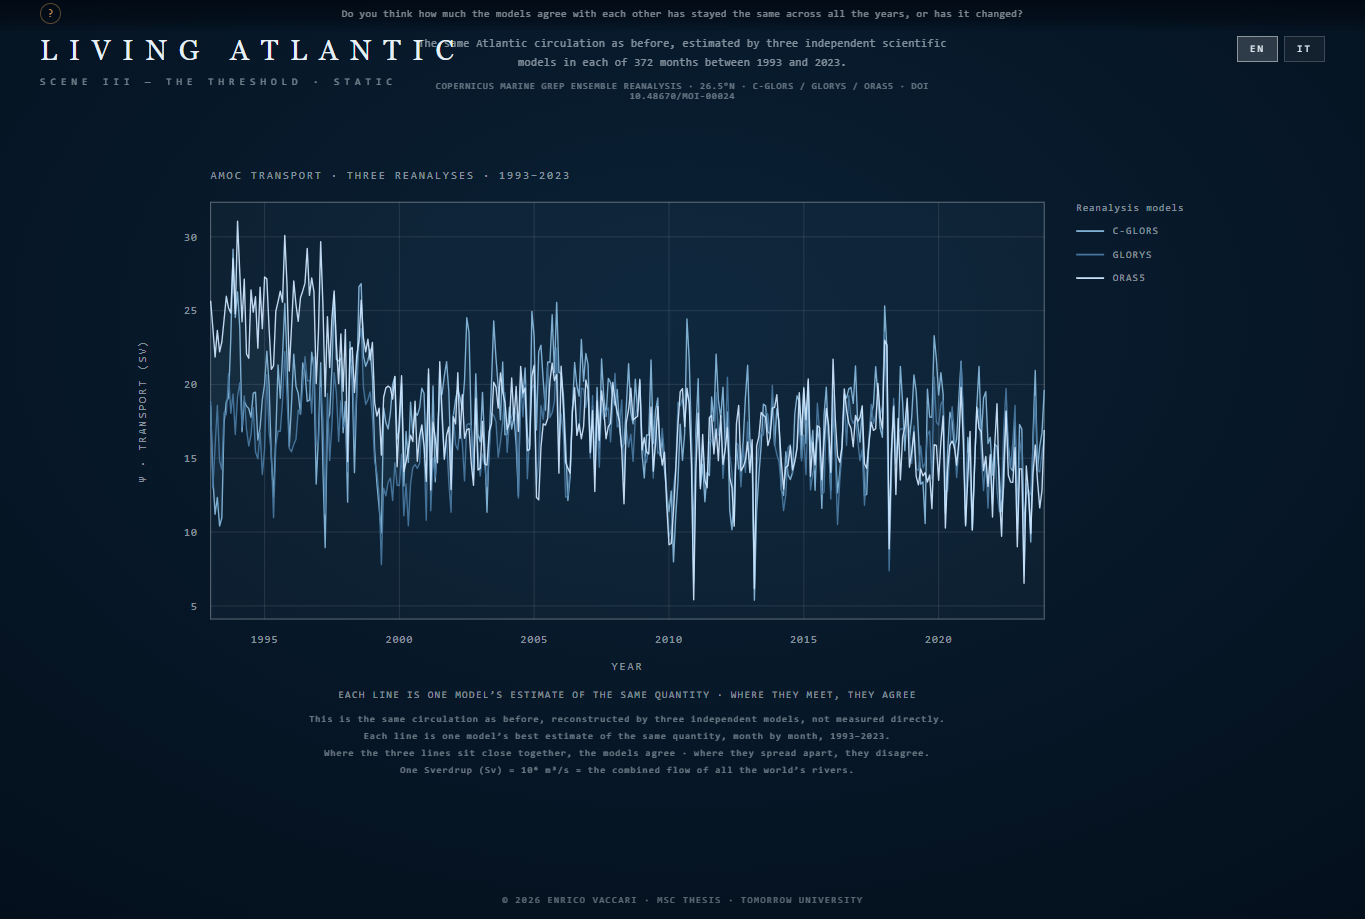
\includegraphics[width=\textwidth]{figures/viz3/viz3_thethreshold-static.png}
    \caption{Control (C1): the static representation of the threshold state.}
    \label{fig:thethreshold-static}
  \end{subfigure}
  \hfill
  \begin{subfigure}[t]{0.48\textwidth}
    \vspace{0pt}
    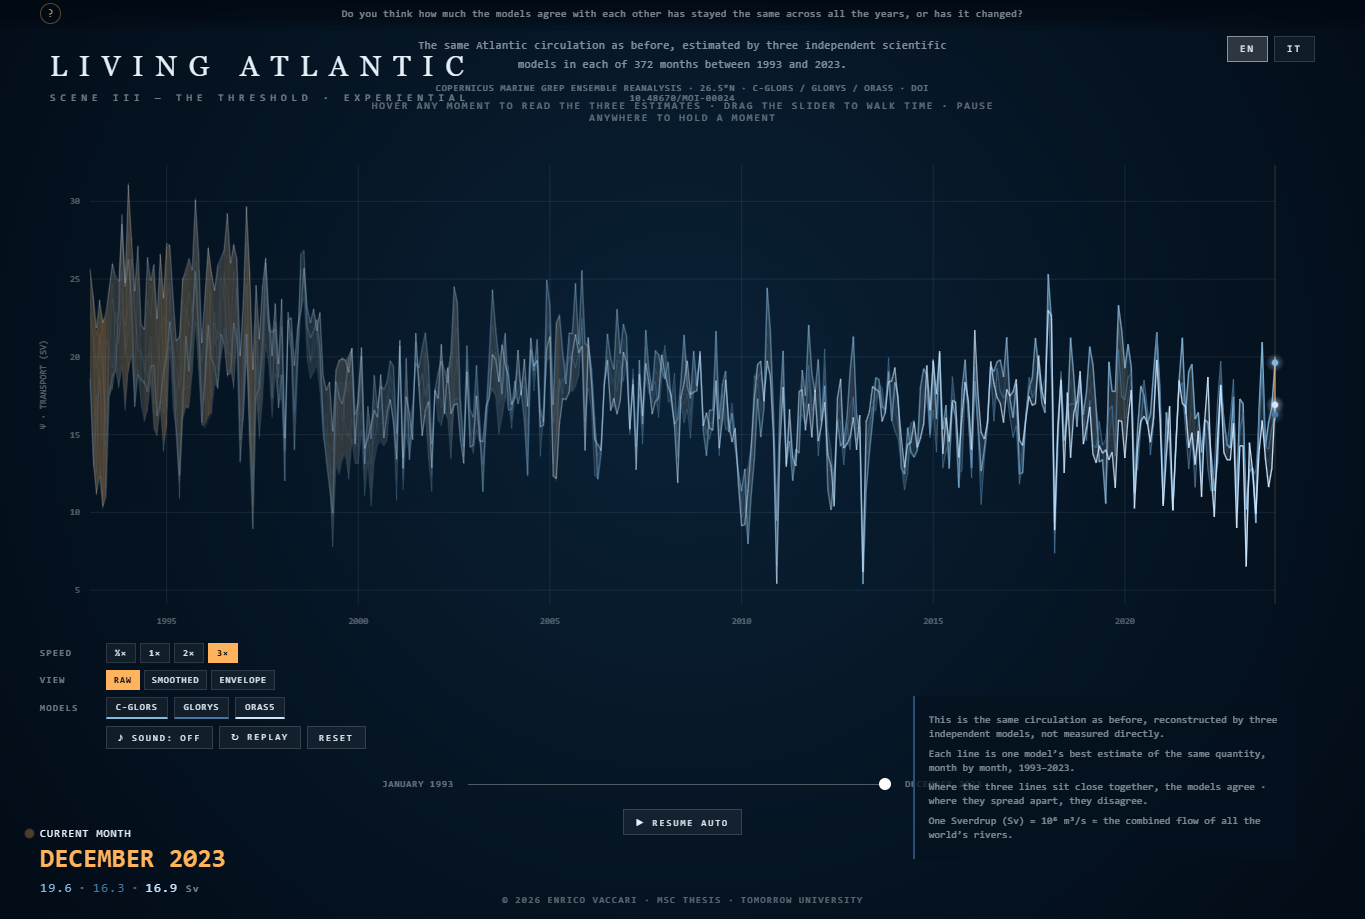
\includegraphics[width=\textwidth]{figures/viz3/viz3_thethreshold-experiential.png}
    \caption{Experiential (C2+C3): the evolving representation of uncertainty beyond the threshold.}
    \label{fig:thethreshold-experiential}
  \end{subfigure}

  \caption[The two conditions of Scene~III]{The two administered conditions of
  Scene~III, generated from the same data bundle through the same reconstruction
  function. The static condition presents the threshold structure as a fixed
  representation, while the experiential condition reveals the divergence and
  evolution of possible trajectories.}

  \label{fig:thethreshold-conditions}
\end{figure}